% answers.tex —— 2013 年·天津卷·理科 · 参考答案与详细解析片段
% 由 tools/generate_projects.py 依来源总账自 2013/2013_数学真题_天津理_试题.md + 2013/2013_数学真题_天津理_解析正文.md + 2013/2013_数学真题_天津理_答案要点.md 生成，勿手改（改源 MD 后重跑）


\begin{answer}
\gksolhead{1}{}

\textbf{题目}：

已知集合 $A=\{x\in\mathbf{R}\mid |x|\leqslant 2\}$，$B=\{x\in\mathbf{R}\mid x\leqslant 1\}$，则 $A\cap B=$\mbox{（　　）}

（A）$(-\infty,2]$；（B）$[1,2]$；（C）$[-2,2]$；（D）$[-2,1]$。

\Needspace{4\baselineskip}
\textbf{解析}
\Needspace{5\baselineskip}
由 $|x|\leqslant 2$ 得
\nopagebreak[4]
\[-2\leqslant x\leqslant 2,\]
\Needspace{5\baselineskip}
故 $A=[-2,2]$。又 $B=(-\infty,1]$，所以
\nopagebreak[4]
\[A\cap B=[-2,1].\]
选 D。

\gkanswer{答案：D。由 $|x|\leqslant2$ 得 $-2\leqslant x\leqslant2$，与 $x\leqslant1$ 取交集得 $[-2,1]$。}

\end{answer}
\begin{answer}
\gksolhead{2}{}

\textbf{题目}：

\Needspace{5\baselineskip}
设变量 $x$，$y$ 满足约束条件
\nopagebreak[4]
\[\begin{cases}
3x+y-6\geqslant 0,\\
x-y-2\leqslant 0,\\
y-3\leqslant 0,
\end{cases}\]
则目标函数 $z=y-2x$ 的最小值为\mbox{（　　）}

（A）$-7$；（B）$-4$；（C）$1$；（D）$2$。

\Needspace{4\baselineskip}
\textbf{解析}
\Needspace{5\baselineskip}
三条边界直线为
\nopagebreak[4]
\[l_1:3x+y-6=0,\qquad l_2:x-y-2=0,\qquad l_3:y=3.\]
\Needspace{5\baselineskip}
两两求交：
\nopagebreak[4]
\[l_1\cap l_2:\ (2,0),\qquad
l_1\cap l_3:\ (1,3),\qquad
l_2\cap l_3:\ (5,3).\]
\Needspace{5\baselineskip}
约束 $y\geqslant 6-3x$，$y\geqslant x-2$，$y\leqslant 3$ 所围可行域是以这三点为顶点的三角形。分别代入 $z=y-2x$：
\nopagebreak[4]
\[z(2,0)=-4,\qquad z(1,3)=1,\qquad z(5,3)=3-10=-7.\]
故最小值为 $-7$，在 $(5,3)$ 处取得。选 A。

\gkanswer{答案：A。可行域顶点为 $(1,3)$，$(5,3)$，$(2,0)$，对应 $z=y-2x$ 的值为 $1$，$-7$，$-4$，最小值为 $-7$。}

\end{answer}
\begin{answer}
\gksolhead{3}{}

\textbf{题目}：

阅读如图的程序框图，运行相应的程序，若输入 $x$ 的值为 $1$，则输出 $S$ 的值为\mbox{（　　）}
\nopagebreak[4]
\begin{center}% ============================================================
% f2013_tianjin_science_q03_flowchart.tex
% 2013 天津卷（理科）第 3 题 程序框图（TikZ 矢量重绘）
% 逻辑：输入 x → S=0 → S=S+x^3 → 判断 S>=50?
%       否 → x=2x → 回到 S=S+x^3；是 → 输出 S → 结束
% ============================================================
\begin{tikzpicture}[
  x=1cm, y=1cm, scale=0.8, transform shape,
  every node/.style={font=\small, inner sep=1pt},
  box/.style={draw, line width=0.6pt, minimum height=0.8cm, align=center},
  arr/.style={-{Stealth[length=2.4mm,width=1.8mm]}, line width=0.6pt},
]

  % ---------- 主干 ----------
  \draw[arr] (0,9.80) -- (0,9.02);
  \draw[arr] (0,8.18) -- (0,7.48);
  \draw[arr] (0,6.72) -- (0,5.92);
  \draw[arr] (0,5.10) -- (0,4.62);
  \draw[arr] (0,2.98) -- (0,2.22);
  \draw[arr] (0,1.38) -- (0,0.74);

  % ---------- 「否」支：菱形右顶点 → 右 → 上 → x=2x ----------
  \draw[arr] (2.90,3.80) -- (4.60,3.80) -- (4.60,5.88);

  % ---------- 回代：x=2x 左侧 → 左 → 下，汇入主干 ----------
  \draw[arr] (3.64,6.30) -- (0,6.30) -- (0,5.92);

  % ---------- 节点 ----------
  \node[box, rounded corners=4pt, minimum width=2.6cm] at (0,10.22) {开始};

  \draw[line width=0.6pt]
    (-1.80,8.18) -- (1.80,8.18) -- (1.42,9.02) -- (-1.42,9.02) -- cycle;
  \node at (0,8.60) {输入 $x$};

  \node[box, minimum width=2.2cm] at (0,7.10) {$S=0$};

  \node[box, minimum width=3.8cm] at (0,5.50) {$S=S+x^3$};

  \draw[line width=0.6pt]
    (0,4.62) -- (2.90,3.80) -- (0,2.98) -- (-2.90,3.80) -- cycle;
  \node at (0,3.80) {$S\geqslant 50$?};

  \draw[line width=0.6pt]
    (-1.70,1.38) -- (1.70,1.38) -- (1.38,2.22) -- (-1.38,2.22) -- cycle;
  \node at (0,1.80) {输出 $S$};

  \node[box, rounded corners=4pt, minimum width=2.4cm] at (0,0.34) {结束};

  \node[box, minimum width=1.9cm] at (4.60,6.30) {$x=2x$};

  % ---------- 分支标注 ----------
  \node at (0.34,2.58) {是};
  \node at (3.55,4.02) {否};

\end{tikzpicture}
\end{center}
\nopagebreak[4]
（A）$64$；（B）$73$；（C）$512$；（D）$585$。

\Needspace{4\baselineskip}
\textbf{解析}
初值 $x=1$，$S=0$。每轮先执行 $S=S+x^3$，再判断 $S\geqslant 50$；若否，执行 $x=2x$ 后回到 $S=S+x^3$。

\begin{center}
\begin{tabular}{llll}
\toprule
轮次 & 进入时 $x$ & 执行 $S=S+x^3$ 后 & 判断 $S\geqslant 50$ \\
\midrule
1 & $1$ & $S=0+1^3=1$ & 否，$x\leftarrow 2$ \\
2 & $2$ & $S=1+2^3=9$ & 否，$x\leftarrow 4$ \\
3 & $4$ & $S=9+4^3=73$ & 是，输出 $S$ \\
\bottomrule
\end{tabular}
\end{center}

故输出 $S=73$。选 B。

\gkanswer{答案：B。逐轮计算：$x=1$ 时 $S=1$；$x=2$ 时 $S=9$；$x=4$ 时 $S=73\geqslant50$，输出 $73$。}

\end{answer}
\begin{answer}
\gksolhead{4}{}

\textbf{题目}：

已知下列三个命题：

① 若一个球的半径缩小到原来的 $\dfrac12$，则其体积缩小到原来的 $\dfrac18$；

② 若两组数据的平均数相等，则它们的标准差也相等；

③ 直线 $x+y+1=0$ 与圆 $x^2+y^2=\dfrac12$ 相切。

其中真命题的序号是\mbox{（　　）}

（A）①②③；（B）①②；（C）①③；（D）②③。

\Needspace{4\baselineskip}
\textbf{解析}
\Needspace{5\baselineskip}
① 球的体积 $V=\dfrac43\pi r^3$。半径变为原来的 $\dfrac12$ 时，
\nopagebreak[4]
\[V'=\frac43\pi\left(\frac r2\right)^3=\frac18\cdot\frac43\pi r^3=\frac18V,\]
体积缩小到原来的 $\dfrac18$，真命题。

② 平均数相等不能推出标准差相等。例如数据 $0,0$ 与 $-1,1$ 的平均数都为 $0$，但标准差分别为 $0$ 与 $1$，假命题。

\Needspace{5\baselineskip}
③ 圆心到直线 $x+y+1=0$ 的距离为
\nopagebreak[4]
\[d=\frac{|0+0+1|}{\sqrt{1^2+1^2}}=\frac1{\sqrt2},\]
而圆 $x^2+y^2=\dfrac12$ 的半径 $r=\dfrac1{\sqrt2}$，故 $d=r$，直线与圆相切，真命题。

所以真命题为①③。选 C。

\gkanswer{答案：C。①体积按半径立方缩放，正确；②平均数相等推不出标准差相等，错误；③圆心到直线距离 $\dfrac1{\sqrt2}$ 等于半径，正确。故为①③。}

\end{answer}
\begin{answer}
\gksolhead{5}{}

\textbf{题目}：

已知双曲线 $\dfrac{x^2}{a^2}-\dfrac{y^2}{b^2}=1$（$a>0$，$b>0$）的两条渐近线与抛物线 $y^2=2px$（$p>0$）的准线分别交于 $A$，$B$ 两点，$O$ 为坐标原点。若双曲线的离心率为 $2$，$\triangle AOB$ 的面积为 $\sqrt3$，则 $p=$\mbox{（　　）}

（A）$1$；（B）$\dfrac32$；（C）$2$；（D）$3$。

\Needspace{4\baselineskip}
\textbf{解析}
\Needspace{5\baselineskip}
双曲线离心率 $e=2$，即 $c=2a$，于是
\nopagebreak[4]
\[b^2=c^2-a^2=4a^2-a^2=3a^2,\]
\Needspace{5\baselineskip}
故渐近线为
\nopagebreak[4]
\[y=\pm\frac ba x=\pm\sqrt3\,x.\]
\Needspace{5\baselineskip}
抛物线 $y^2=2px$ 的准线为 $x=-\dfrac p2$。代入渐近线得
\nopagebreak[4]
\[A\left(-\frac p2,\frac{\sqrt3p}{2}\right),\qquad
B\left(-\frac p2,-\frac{\sqrt3p}{2}\right),\]
\Needspace{5\baselineskip}
所以
\nopagebreak[4]
\[|AB|=\sqrt3p.\]
\Needspace{5\baselineskip}
原点 $O$ 到准线 $x=-\dfrac p2$ 的距离为 $\dfrac p2$，故
\nopagebreak[4]
\[S_{\triangle AOB}=\frac12\cdot\sqrt3p\cdot\frac p2=\frac{\sqrt3p^2}{4}.\]
\Needspace{5\baselineskip}
由 $S_{\triangle AOB}=\sqrt3$ 得
\nopagebreak[4]
\[\frac{\sqrt3p^2}{4}=\sqrt3\Longrightarrow p^2=4\Longrightarrow p=2\quad(p>0).\]
选 C。

\gkanswer{答案：C。由 $e=2$ 得 $b^2=3a^2$，渐近线 $y=\pm\sqrt3x$ 与准线 $x=-\dfrac p2$ 交出 $|AB|=\sqrt3p$，故 $S_{\triangle AOB}=\dfrac{\sqrt3p^2}{4}=\sqrt3$，得 $p=2$。}

\end{answer}
\begin{answer}
\gksolhead{6}{}

\textbf{题目}：

在 $\triangle ABC$ 中，$\angle ABC=\dfrac{\pi}{4}$，$AB=\sqrt2$，$BC=3$，则 $\sin\angle BAC=$\mbox{（　　）}

（A）$\dfrac{\sqrt{10}}{10}$；（B）$\dfrac{\sqrt{10}}{5}$；（C）$\dfrac{3\sqrt{10}}{10}$；（D）$\dfrac{\sqrt5}{5}$。

\Needspace{4\baselineskip}
\textbf{解析}
\Needspace{5\baselineskip}
在 $\triangle ABC$ 中，由余弦定理
\nopagebreak[4]
\[\begin{aligned}
AC^2&=AB^2+BC^2-2\cdot AB\cdot BC\cos\angle ABC\\
&=2+9-2\cdot\sqrt2\cdot3\cdot\frac{\sqrt2}{2}\\
&=11-6=5,
\end{aligned}\]
故 $AC=\sqrt5$。

\Needspace{5\baselineskip}
再由正弦定理
\nopagebreak[4]
\[\frac{BC}{\sin\angle BAC}=\frac{AC}{\sin\angle ABC},\]
\Needspace{5\baselineskip}
得
\nopagebreak[4]
\[\sin\angle BAC=\frac{BC\sin\angle ABC}{AC}
=\frac{3\cdot\frac{\sqrt2}{2}}{\sqrt5}
=\frac{3}{\sqrt{10}}
=\frac{3\sqrt{10}}{10}.\]
选 C。

\gkanswer{答案：C。由余弦定理 $AC^2=2+9-6=5$，再由正弦定理 $\sin\angle BAC=\dfrac{3\sin45^\circ}{\sqrt5}=\dfrac{3\sqrt{10}}{10}$。}

\end{answer}
\begin{answer}
\gksolhead{7}{}

\textbf{题目}：

函数 $f(x)=2^x|\log_{0.5}x|-1$ 的零点个数为\mbox{（　　）}

（A）$1$；（B）$2$；（C）$3$；（D）$4$。

\Needspace{4\baselineskip}
\textbf{解析}
\Needspace{5\baselineskip}
定义域为 $x>0$。因为
\nopagebreak[4]
\[|\log_{0.5}x|=|-\log_2x|=|\log_2x|,\]
\Needspace{5\baselineskip}
所以
\nopagebreak[4]
\[f(x)=2^x|\log_2x|-1.\]

\Needspace{5\baselineskip}
当 $0<x<1$ 时，$\log_2x<0$，于是
\nopagebreak[4]
\[f(x)=-2^x\log_2x-1.\]
\Needspace{5\baselineskip}
求导：
\nopagebreak[4]
\[f'(x)=2^x\ln2\cdot(-\log_2x)-\frac{2^x}{x\ln2}<0,\]
\Needspace{5\baselineskip}
故 $f$ 在 $(0,1)$ 上严格递减；又
\nopagebreak[4]
\[\lim_{x\to0^+}f(x)=+\infty,\qquad f(1)=-1,\]
所以 $f$ 在 $(0,1)$ 内恰有一个零点。

\Needspace{5\baselineskip}
当 $x>1$ 时，$\log_2x>0$，于是
\nopagebreak[4]
\[f(x)=2^x\log_2x-1,\]
\nopagebreak[4]
\[f'(x)=2^x\ln2\cdot\log_2x+\frac{2^x}{x\ln2}>0,\]
\Needspace{5\baselineskip}
故 $f$ 在 $(1,+\infty)$ 上严格递增；又
\nopagebreak[4]
\[f(1)=-1,\qquad f(2)=4-1=3>0,\]
所以 $f$ 在 $(1,+\infty)$ 内恰有一个零点。

两段合计，零点个数为 $2$。选 B。

\gkanswer{答案：B。$0<x<1$ 时 $f$ 严格递减且由 $+\infty$ 降至 $-1$，有一个零点；$x>1$ 时 $f$ 严格递增且由 $-1$ 升至 $+\infty$，有一个零点；共 $2$ 个。}

\end{answer}
\begin{answer}
\gksolhead{8}{}

\textbf{题目}：

已知函数 $f(x)=x(1+a|x|)$。设关于 $x$ 的不等式 $f(x+a)<f(x)$ 的解集为 $A$，若 $\left[-\dfrac12,\dfrac12\right]\subseteq A$，则实数 $a$ 的取值范围是\mbox{（　　）}

（A）$\left(\dfrac{1-\sqrt5}{2},0\right)$；（B）$\left(\dfrac{1-\sqrt3}{2},0\right)$；（C）$\left(\dfrac{1-\sqrt5}{2},0\right)\cup\left(0,\dfrac{1+\sqrt3}{2}\right)$；（D）$\left(-\infty,\dfrac{1-\sqrt5}{2}\right)$。

\Needspace{4\baselineskip}
\textbf{解析}
若 $a=0$，则 $f(x)=x$，不等式 $f(x+a)<f(x)$ 化为 $x<x$，无解，不合题意。

\Needspace{5\baselineskip}
若 $a>0$，则
\nopagebreak[4]
\[f'(x)=1+2a|x|>0\quad(x\neq0),\]
且 $f$ 在 $x=0$ 处连续，故 $f$ 在 $\mathbf R$ 上严格递增。于是 $f(x+a)<f(x)$ 等价于 $x+a<x$，即 $a<0$，与 $a>0$ 矛盾。因此必有 $a<0$。

\Needspace{5\baselineskip}
令 $c=-a>0$，则 $a=-c$，需对一切 $x\in\left[-\dfrac12,\dfrac12\right]$ 有
\nopagebreak[4]
\[f(x-c)<f(x).\]

\Needspace{5\baselineskip}
当 $-\dfrac12\leqslant x\leqslant0$ 时，$x<0$，$x-c<0$，此时 $f(t)=t+ct^2$，故
\nopagebreak[4]
\[\begin{aligned}
f(x)-f(x-c)
&=\bigl(x+cx^2\bigr)-\bigl[(x-c)+c(x-c)^2\bigr]\\
&=c(1+2cx-c^2).
\end{aligned}\]
\Needspace{5\baselineskip}
右端在 $x\in\left[-\dfrac12,0\right]$ 上关于 $x$ 单调递增，最小值在 $x=-\dfrac12$ 处取得，为
\nopagebreak[4]
\[c(1-c-c^2).\]
\Needspace{5\baselineskip}
要求它恒正，即
\nopagebreak[4]
\[c^2+c-1<0\Longrightarrow 0<c<\frac{\sqrt5-1}{2}.\]

当 $0\leqslant x\leqslant\dfrac12$ 时，$x\geqslant0$，$f(x)=x-cx^2$。

\Needspace{5\baselineskip}
若 $x\leqslant c$，则 $x-c\leqslant0$，直接计算得
\nopagebreak[4]
\[f(x)-f(x-c)=c(1-2x^2+2cx-c^2).\]
\Needspace{5\baselineskip}
括号内关于 $x$ 是开口向下的二次函数，在区间 $[0,c]$ 上的最小值在端点取得；而
\nopagebreak[4]
\[1-0+0-c^2=1-c^2>0,\qquad
1-2c^2+2c^2-c^2=1-c^2>0,\]
故此时恒有 $f(x)>f(x-c)$。

\Needspace{5\baselineskip}
若 $x\geqslant c$，则 $x-c\geqslant0$，同理
\nopagebreak[4]
\[f(x)-f(x-c)=c(1-2cx+c^2).\]
\Needspace{5\baselineskip}
由 $x\leqslant\dfrac12$ 得
\nopagebreak[4]
\[1-2cx+c^2\geqslant 1-c+c^2=\left(c-\frac12\right)^2+\frac34>0.\]

因此当 $0<c<\dfrac{\sqrt5-1}{2}$ 时，题设包含关系成立。反之，若 $c\geqslant\dfrac{\sqrt5-1}{2}$，则在 $x=-\dfrac12$ 处有 $f(x)-f(x-c)\leqslant0$，即 $f\left(-\dfrac12-c\right)\geqslant f\left(-\dfrac12\right)$，不满足 $\left[-\dfrac12,\dfrac12\right]\subseteq A$。

\Needspace{5\baselineskip}
综上，
\nopagebreak[4]
\[0<c<\frac{\sqrt5-1}{2}
\Longleftrightarrow
\frac{1-\sqrt5}{2}<a<0.\]
选 A。

\gkanswer{答案：A。令 $c=-a>0$。由 $x\in\left[-\dfrac12,0\right]$ 的严格不等式得 $c^2+c-1<0$，即 $0<c<\dfrac{\sqrt5-1}{2}$；$x\in\left[0,\dfrac12\right]$ 自动满足。故 $a\in\left(\dfrac{1-\sqrt5}{2},0\right)$。}

\end{answer}
\begin{answer}
\gksolhead{9}{}

\textbf{题目}：

已知 $a$，$b\in\mathbf{R}$，$\mathrm i$ 是虚数单位。若 $(a+\mathrm i)(1+\mathrm i)=b\mathrm i$，则 $a+b\mathrm i=$\gkblank{}。

\Needspace{4\baselineskip}
\textbf{解析}
\Needspace{5\baselineskip}
展开左边：
\nopagebreak[4]
\[(a+\mathrm i)(1+\mathrm i)=a+a\mathrm i+\mathrm i+\mathrm i^2
=(a-1)+(a+1)\mathrm i.\]
\Needspace{5\baselineskip}
与 $b\mathrm i$ 比较实部、虚部：
\nopagebreak[4]
\[a-1=0,\qquad a+1=b.\]
\Needspace{5\baselineskip}
解得 $a=1$，$b=2$，故
\nopagebreak[4]
\[a+b\mathrm i=1+2\mathrm i.\]

\gkanswer{答案：$1+2\mathrm i$。展开得 $(a-1)+(a+1)\mathrm i=b\mathrm i$，故 $a=1$，$b=2$。}

\end{answer}
\begin{answer}
\gksolhead{10}{}

\textbf{题目}：

$\left(x-\dfrac{1}{\sqrt{x}}\right)^6$ 的二项展开式中的常数项为\gkblank{}。

\Needspace{4\baselineskip}
\textbf{解析}
\Needspace{5\baselineskip}
二项展开式的通项为
\nopagebreak[4]
\[T_{k+1}=\mathrm C_6^k x^{6-k}\left(-\frac1{\sqrt x}\right)^k
=\mathrm C_6^k(-1)^k x^{6-\frac{3k}{2}}\quad(k=0,1,\dots,6).\]
\Needspace{5\baselineskip}
令 $x$ 的指数为零：
\nopagebreak[4]
\[6-\frac{3k}{2}=0\Longrightarrow k=4.\]
\Needspace{5\baselineskip}
故常数项为
\nopagebreak[4]
\[\mathrm C_6^4(-1)^4=15.\]

\gkanswer{答案：$15$。通项为 $\mathrm C_6^k(-1)^kx^{6-\frac{3k}{2}}$，令 $6-\dfrac{3k}{2}=0$ 得 $k=4$，常数项为 $\mathrm C_6^4=15$。}

\end{answer}
\begin{answer}
\gksolhead{11}{}

\textbf{题目}：

已知圆的极坐标方程为 $\rho=4\cos\theta$，圆心为 $C$，点 $P$ 的极坐标为 $\left(4,\dfrac{\pi}{3}\right)$，则 $|CP|=$\gkblank{}。

\Needspace{4\baselineskip}
\textbf{解析}
\Needspace{5\baselineskip}
由 $\rho=4\cos\theta$ 得
\nopagebreak[4]
\[\rho^2=4\rho\cos\theta\Longrightarrow x^2+y^2=4x,\]
\Needspace{5\baselineskip}
即
\nopagebreak[4]
\[(x-2)^2+y^2=4,\]
圆心 $C(2,0)$。

\Needspace{5\baselineskip}
点 $P$ 的直角坐标为
\nopagebreak[4]
\[x_P=4\cos\frac\pi3=2,\qquad y_P=4\sin\frac\pi3=2\sqrt3,\]
\Needspace{5\baselineskip}
即 $P(2,2\sqrt3)$。于是
\nopagebreak[4]
\[|CP|=\sqrt{(2-2)^2+(2\sqrt3-0)^2}=2\sqrt3.\]

\gkanswer{答案：$2\sqrt3$。圆的直角坐标方程为 $(x-2)^2+y^2=4$，圆心 $C(2,0)$；$P$ 的直角坐标为 $(2,2\sqrt3)$，故 $|CP|=2\sqrt3$。}

\end{answer}
\begin{answer}
\gksolhead{12}{}

\textbf{题目}：

在平行四边形 $ABCD$ 中，$AD=1$，$\angle BAD=60^\circ$，$E$ 为 $CD$ 的中点。若 $\overrightarrow{AC}\cdot\overrightarrow{BE}=1$，则 $AB$ 的长为\gkblank{}。

\Needspace{4\baselineskip}
\textbf{解析}
\Needspace{5\baselineskip}
设 $\overrightarrow{AB}=\boldsymbol a$，$\overrightarrow{AD}=\boldsymbol b$，则
\nopagebreak[4]
\[|\boldsymbol b|=1,\qquad \boldsymbol a\cdot\boldsymbol b=|\boldsymbol a|\cdot1\cdot\cos60^\circ=\frac{|\boldsymbol a|}{2}.\]
\Needspace{5\baselineskip}
由平行四边形法则，
\nopagebreak[4]
\[\overrightarrow{AC}=\boldsymbol a+\boldsymbol b.\]
\Needspace{5\baselineskip}
又 $E$ 为 $CD$ 的中点，$C=\boldsymbol a+\boldsymbol b$，$D=\boldsymbol b$，故
\nopagebreak[4]
\[\overrightarrow{AE}=\frac{\overrightarrow{AC}+\overrightarrow{AD}}2
=\frac{\boldsymbol a+2\boldsymbol b}{2}
=\frac{\boldsymbol a}{2}+\boldsymbol b,\]
\Needspace{5\baselineskip}
从而
\nopagebreak[4]
\[\overrightarrow{BE}=\overrightarrow{AE}-\overrightarrow{AB}
=-\frac{\boldsymbol a}{2}+\boldsymbol b.\]
\Needspace{5\baselineskip}
于是
\nopagebreak[4]
\[\begin{aligned}
\overrightarrow{AC}\cdot\overrightarrow{BE}
&=(\boldsymbol a+\boldsymbol b)\cdot\left(-\frac{\boldsymbol a}{2}+\boldsymbol b\right)\\
&=-\frac{|\boldsymbol a|^2}{2}+\boldsymbol a\cdot\boldsymbol b
-\frac{\boldsymbol a\cdot\boldsymbol b}{2}+|\boldsymbol b|^2\\
&=-\frac{|\boldsymbol a|^2}{2}+\frac{|\boldsymbol a|}{4}+1.
\end{aligned}\]
\Needspace{5\baselineskip}
由题设该值为 $1$，得
\nopagebreak[4]
\[-\frac{|\boldsymbol a|^2}{2}+\frac{|\boldsymbol a|}{4}=0
\Longrightarrow |\boldsymbol a|\left(\frac14-\frac{|\boldsymbol a|}{2}\right)=0.\]
\Needspace{5\baselineskip}
因 $|\boldsymbol a|>0$，故
\nopagebreak[4]
\[|\boldsymbol a|=\frac12,\]
即 $AB=\dfrac12$。

\gkanswer{答案：$\dfrac12$。设 $\overrightarrow{AB}=\boldsymbol a$，$\overrightarrow{AD}=\boldsymbol b$，由 $\overrightarrow{AC}\cdot\overrightarrow{BE}=-\dfrac{|\boldsymbol a|^2}{2}+\dfrac{|\boldsymbol a|}{4}+1=1$ 得 $|\boldsymbol a|=\dfrac12$。}

\end{answer}
\begin{answer}
\gksolhead{13}{}

\textbf{题目}：

如图，$\triangle ABC$ 为圆的内接三角形，$BD$ 为圆的弦，且 $BD\parallel AC$。过点 $A$ 作圆的切线与 $DB$ 的延长线交于点 $E$，$AD$ 与 $BC$ 交于点 $F$。若 $AB=AC$，$AE=6$，$BD=5$，则线段 $CF$ 的长为\gkblank{}。
\nopagebreak[4]
\begin{center}% ============================================================
% f2013_tianjin_science_q13_circle.tex
% 2013 天津卷（理科）第 13 题 圆内接三角形与切线（TikZ 矢量重绘）
% 几何：圆 O，A 在圆上；AB=AC；BD∥AC，E 在 DB 延长线上，EA 切圆于 A；
%       AD 与 BC 交于 F。图中坐标按题设 AE=6、BD=5、AB=AC 精确构造后缩放。
% ============================================================
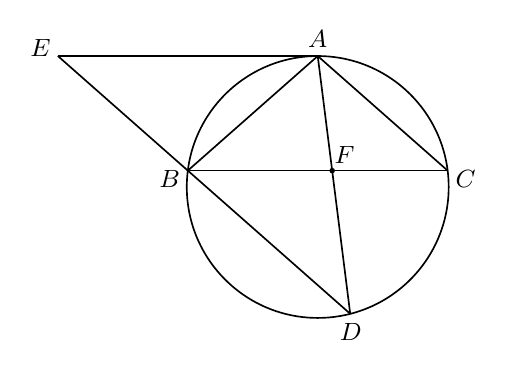
\begin{tikzpicture}[
  x=1cm, y=1cm,
  every node/.style={font=\small, inner sep=1pt},
  line/.style={line width=0.6pt},
]

  % 圆：R = 8/sqrt(7) * 0.55
  \draw[line] (0,0) circle [radius=1.6630];

  % 切线 EA 与割线 E-B-D
  \draw[line] (-3.30,1.6630) -- (0,1.6630);
  \draw[line] (-3.30,1.6630) -- (0.4125,-1.6105);

  % 三角形 ABC 与弦 AD
  \draw[line] (0,1.6630) -- (-1.6500,0.2078);
  \draw[line] (0,1.6630) -- (1.6500,0.2078);
  \draw[line] (-1.6500,0.2078) -- (1.6500,0.2078);
  \draw[line] (0,1.6630) -- (0.4125,-1.6105);

  % 交点 F
  \fill (0.1833,0.2078) circle [radius=0.035];

  % 标签
  \node at (0,1.88) {$A$};
  \node at (-1.88,0.10) {$B$};
  \node at (1.88,0.10) {$C$};
  \node at (0.42,-1.84) {$D$};
  \node at (-3.52,1.76) {$E$};
  \node at (0.34,0.40) {$F$};

\end{tikzpicture}
\end{center}
\nopagebreak[4]
\Needspace{4\baselineskip}
\textbf{解析}
\Needspace{5\baselineskip}
由切割线定理，
\nopagebreak[4]
\[EA^2=EB\cdot ED.\]
\Needspace{5\baselineskip}
又 $E$，$B$，$D$ 共线且 $B$ 在 $E$，$D$ 之间，
\nopagebreak[4]
\[ED=EB+BD=EB+5.\]
\Needspace{5\baselineskip}
代入 $EA=6$：
\nopagebreak[4]
\[36=EB(EB+5)\Longrightarrow EB^2+5EB-36=0
\Longrightarrow EB=4\quad(EB>0),\]
从而 $ED=9$。

\Needspace{5\baselineskip}
下面证明 $\triangle EAB\sim\triangle BCA$。由弦切角定理，
\nopagebreak[4]
\[\angle EAB=\angle ADB.\]
\Needspace{5\baselineskip}
又 $A$，$B$，$D$，$C$ 四点共圆，$\angle ADB$ 与 $\angle ACB$ 同对弧 $AB$，故
\nopagebreak[4]
\[\angle ADB=\angle ACB,\]
\Needspace{5\baselineskip}
于是
\nopagebreak[4]
\[\angle EAB=\angle ACB.\]
\Needspace{5\baselineskip}
再由 $BD\parallel AC$ 及 $E$，$B$，$D$ 共线，
\nopagebreak[4]
\[\angle EBA=180^\circ-\angle ABD.\]
\Needspace{5\baselineskip}
而 $BD\parallel AC$，射线 $BA$ 与 $AC$ 的夹角为 $180^\circ-\angle BAC$，即
\nopagebreak[4]
\[\angle ABD=180^\circ-\angle BAC,\]
\Needspace{5\baselineskip}
所以
\nopagebreak[4]
\[\angle EBA=\angle BAC.\]
\Needspace{5\baselineskip}
因此 $\triangle EAB\sim\triangle BCA$，对应边成比例：
\nopagebreak[4]
\[\frac{EA}{BC}=\frac{AB}{CA}=\frac{EB}{AB}.\]
\Needspace{5\baselineskip}
由 $AB=AC$ 得 $\dfrac{AB}{CA}=1$，故
\nopagebreak[4]
\[BC=EA=6,\qquad AB=EB=4.\]

\Needspace{5\baselineskip}
又 $ABDC$ 为圆内接梯形（$BD\parallel AC$），两腰相等，故
\nopagebreak[4]
\[CD=AB=4.\]
\Needspace{5\baselineskip}
由托勒密定理
\nopagebreak[4]
\[AB\cdot CD+AC\cdot BD=AD\cdot BC,\]
\Needspace{5\baselineskip}
即
\nopagebreak[4]
\[4\cdot4+4\cdot5=6AD\Longrightarrow AD=6.\]
\Needspace{5\baselineskip}
设 $CF=x$，则 $BF=BC-CF=6-x$。由 $A$，$B$，$C$，$D$ 四点共圆，
\nopagebreak[4]
\[\angle FBD=\angle CBD=\angle CAD=\angle FAC,\]
\nopagebreak[4]
\[\angle FDB=\angle ADB=\angle ACB=\angle FCA,\]
\Needspace{5\baselineskip}
故
\nopagebreak[4]
\[\triangle FBD\sim\triangle FAC,\]
\Needspace{5\baselineskip}
于是
\nopagebreak[4]
\[\frac{BF}{AF}=\frac{FD}{FC}=\frac{BD}{AC}=\frac54.\]
\Needspace{5\baselineskip}
于是
\nopagebreak[4]
\[FD=\frac54x,\qquad AF=AD-FD=6-\frac54x.\]
\Needspace{5\baselineskip}
代入 $\dfrac{BF}{AF}=\dfrac54$：
\nopagebreak[4]
\[\frac{6-x}{6-\frac54x}=\frac54.\]
\Needspace{5\baselineskip}
去分母：
\nopagebreak[4]
\[4(6-x)=5\left(6-\frac54x\right)
\Longrightarrow 24-4x=30-\frac{25}{4}x.\]
\Needspace{5\baselineskip}
两边乘以 $4$：
\nopagebreak[4]
\[96-16x=120-25x\Longrightarrow 9x=24
\Longrightarrow x=\frac83.\]
\Needspace{5\baselineskip}
故
\nopagebreak[4]
\[CF=\frac83.\]

\gkanswer{答案：$\dfrac83$。切割线定理得 $EB=4$，$ED=9$；由弦切角与 $BD\parallel AC$ 得 $\triangle EAB\sim\triangle BCA$，故 $AB=4$，$BC=6$；再由 $\triangle FBD\sim\triangle FAC$ 得 $\dfrac{BF}{AF}=\dfrac{FD}{FC}=\dfrac54$，结合 $BF+FC=6$、$AD=6$ 解得 $FC=\dfrac83$。}

\end{answer}
\begin{answer}
\gksolhead{14}{}

\textbf{题目}：

设 $a+b=2$，$b>0$，则当 $a=$\gkblank{}时，$\dfrac{1}{2|a|}+\dfrac{|a|}{b}$ 取得最小值。

\Needspace{4\baselineskip}
\textbf{解析}
记 $u=|a|>0$，则 $b=2-a$。

\Needspace{5\baselineskip}
若 $a>0$，则 $0<a<2$，$b=2-a>0$，目标式为
\nopagebreak[4]
\[F(a)=\frac1{2a}+\frac{a}{2-a}.\]
\Needspace{5\baselineskip}
求导：
\nopagebreak[4]
\[F'(a)=-\frac1{2a^2}+\frac{2}{(2-a)^2}.\]
\Needspace{5\baselineskip}
令 $F'(a)=0$，得
\nopagebreak[4]
\[(2-a)^2=4a^2\Longrightarrow 2-a=2a\Longrightarrow a=\frac23,\]
\Needspace{5\baselineskip}
此时
\nopagebreak[4]
\[F\left(\frac23\right)=\frac34+\frac{2/3}{4/3}=\frac34+\frac12=\frac54.\]

\Needspace{5\baselineskip}
若 $a<0$，令 $u=-a>0$，则 $b=2+u$，目标式为
\nopagebreak[4]
\[G(u)=\frac1{2u}+\frac{u}{2+u}.\]
\Needspace{5\baselineskip}
求导：
\nopagebreak[4]
\[G'(u)=-\frac1{2u^2}+\frac{2}{(2+u)^2}.\]
\Needspace{5\baselineskip}
令 $G'(u)=0$，得
\nopagebreak[4]
\[(2+u)^2=4u^2\Longrightarrow 2+u=2u\Longrightarrow u=2,\]
\Needspace{5\baselineskip}
即 $a=-2$，此时
\nopagebreak[4]
\[G(2)=\frac14+\frac24=\frac34.\]

比较 $\dfrac34<\dfrac54$，故最小值为 $\dfrac34$，在 $a=-2$ 时取得。

\gkanswer{答案：$-2$。$a>0$ 时最小值 $\dfrac54$（$a=\dfrac23$）；$a<0$ 时最小值 $\dfrac34$（$a=-2$）。故取 $a=-2$。}

\end{answer}
\begin{answer}
\gksolhead{15}{}

\textbf{题目}：

已知函数 $f(x)=-\sqrt2\sin\left(2x+\dfrac{\pi}{4}\right)+6\sin x\cos x-2\cos^2x+1$，$x\in\mathbf{R}$。

（1） 求 $f(x)$ 的最小正周期；

（2） 求 $f(x)$ 在区间 $\left[0,\dfrac{\pi}{2}\right]$ 上的最大值和最小值。

\Needspace{4\baselineskip}
\textbf{解析}
\Needspace{5\baselineskip}
\textbf{（1）} 先化简。由辅助角公式，
\nopagebreak[4]
\[-\sqrt2\sin\left(2x+\frac\pi4\right)
=-\sqrt2\left(\sin2x\cos\frac\pi4+\cos2x\sin\frac\pi4\right)
=-(\sin2x+\cos2x).\]
\Needspace{5\baselineskip}
又
\nopagebreak[4]
\[6\sin x\cos x=3\sin2x,\qquad
-2\cos^2x+1=-\cos2x.\]
\Needspace{5\baselineskip}
所以
\nopagebreak[4]
\[\begin{aligned}
f(x)
&=-(\sin2x+\cos2x)+3\sin2x-\cos2x\\
&=2\sin2x-2\cos2x\\
&=2\sqrt2\sin\left(2x-\frac\pi4\right).
\end{aligned}\]
\Needspace{5\baselineskip}
故最小正周期为
\nopagebreak[4]
\[T=\frac{2\pi}{2}=\pi.\]

\Needspace{5\baselineskip}
\textbf{（2）} 当 $0\leqslant x\leqslant\dfrac\pi2$ 时，
\nopagebreak[4]
\[-\frac\pi4\leqslant 2x-\frac\pi4\leqslant\frac{3\pi}{4}.\]
\Needspace{5\baselineskip}
在此区间上，
\nopagebreak[4]
\[-\frac{\sqrt2}{2}\leqslant\sin\left(2x-\frac\pi4\right)\leqslant1.\]
\Needspace{5\baselineskip}
于是
\nopagebreak[4]
\[-2\leqslant f(x)\leqslant2\sqrt2.\]
当 $2x-\dfrac\pi4=\dfrac\pi2$，即 $x=\dfrac{3\pi}{8}$ 时，$f(x)$ 取得最大值 $2\sqrt2$；当 $2x-\dfrac\pi4=-\dfrac\pi4$，即 $x=0$ 时，$f(x)$ 取得最小值 $-2$。

\gkanswer{答案（1）：$\pi$。化简得 $f(x)=2\sqrt2\sin\left(2x-\dfrac\pi4\right)$，故最小正周期为 $\pi$。}

\gkanswer{答案（2）：最大值 $2\sqrt2$，最小值 $-2$。在 $\left[0,\dfrac\pi2\right]$ 上 $2x-\dfrac\pi4\in\left[-\dfrac\pi4,\dfrac{3\pi}{4}\right]$，故 $f(x)\in[-2,2\sqrt2]$。}

\end{answer}
\begin{answer}
\gksolhead{16}{}

\textbf{题目}：

一个盒子里装有 7 张卡片，其中有红色卡片 4 张，编号分别为 1，2，3，4；白色卡片 3 张，编号分别为 2，3，4。从盒子中任取 4 张卡片（假设取到任何一张卡片的可能性相同）。

（1） 求取出的 4 张卡片中，含有编号为 3 的卡片的概率。

（2） 在取出的 4 张卡片中，红色卡片编号的最大值设为 $X$，求随机变量 $X$ 的分布列和数学期望。

\Needspace{4\baselineskip}
\textbf{解析}
\Needspace{5\baselineskip}
从 $7$ 张卡片中任取 $4$ 张，共有
\nopagebreak[4]
\[\mathrm C_7^4=35\]
种等可能取法。

\Needspace{5\baselineskip}
\textbf{（1）} 用对立事件。不含编号为 $3$ 的卡片时，只能从剩下的 $5$ 张（红 $1,2,4$，白 $2,4$）中取 $4$ 张，共 $\mathrm C_5^4=5$ 种。故
\nopagebreak[4]
\[P(\text{\text{含有编号为} }3\text{ \text{的卡片}})
=1-\frac{5}{35}=\frac67.\]

\textbf{（2）} $X$ 的可能取值为 $1,2,3,4$。因只有 $3$ 张白色卡片，任取 $4$ 张必含红色卡片，故 $X$ 有定义。

\begin{itemize}
\item $X=1$：必须取红 $1$，且不取红 $2,3,4$，其余 $3$ 张只能全取白 $2,3,4$，共 $1$ 种；
\item $X=2$：必须取红 $2$，不取红 $3,4$，再从红 $1$ 与白 $2,3,4$ 共 $4$ 张中取 $3$ 张，共 $\mathrm C_4^3=4$ 种；
\item $X=3$：必须取红 $3$，不取红 $4$，再从其余 $5$ 张中取 $3$ 张，共 $\mathrm C_5^3=10$ 种；
\item $X=4$：必须取红 $4$，再从其余 $6$ 张中取 $3$ 张，共 $\mathrm C_6^3=20$ 种。
\end{itemize}

校验：$1+4+10+20=35$。分布列为

\begin{center}
\begin{tabular}{lllll}
\toprule
$X$ & $1$ & $2$ & $3$ & $4$ \\
\midrule
$P$ & $\dfrac1{35}$ & $\dfrac4{35}$ & $\dfrac{10}{35}$ & $\dfrac{20}{35}$ \\
\bottomrule
\end{tabular}
\end{center}

\Needspace{5\baselineskip}
数学期望为
\nopagebreak[4]
\[\begin{aligned}
E(X)&=1\cdot\frac1{35}+2\cdot\frac4{35}+3\cdot\frac{10}{35}+4\cdot\frac{20}{35}\\
&=\frac{1+8+30+80}{35}
=\frac{119}{35}=\frac{17}{5}.
\end{aligned}\]

\gkanswer{答案（1）：$\dfrac67$。总取法 $\mathrm C_7^4=35$，不含编号 $3$ 的取法为 $\mathrm C_5^4=5$，故所求为 $1-\dfrac5{35}=\dfrac67$。}

\gkanswer{答案（2）：$P(X=1)=\dfrac1{35}$，$P(X=2)=\dfrac4{35}$，$P(X=3)=\dfrac{10}{35}=\dfrac27$，$P(X=4)=\dfrac{20}{35}=\dfrac47$；$E(X)=\dfrac{17}{5}$。计数分别为 $1,4,10,20$，总和 $35$，期望 $\dfrac{1+8+30+80}{35}=\dfrac{17}{5}$。}

\end{answer}
\begin{answer}
\gksolhead{17}{}

\textbf{题目}：

如图所示，在四棱柱 $ABCD\text{-}A_1B_1C_1D_1$ 中，侧棱 $A_1A\perp$ 底面 $ABCD$，$AB\parallel DC$，$AB\perp AD$，$AD=CD=1$，$AA_1=AB=2$，$E$ 为棱 $AA_1$ 的中点。

（1） 证明：$B_1C_1\perp CE$；

（2） 求二面角 $B_1\text{-}CE\text{-}C_1$ 的平面角的正弦值；

（3） 设点 $M$ 在线段 $C_1E$ 上，且直线 $AM$ 与平面 $ADD_1A_1$ 所成角的正弦值为 $\dfrac{\sqrt2}{6}$，求线段 $AM$ 的长。
\nopagebreak[4]
\begin{center}% ============================================================
% f2013_tianjin_science_q17_prism.tex
% 2013 天津卷（理科）第 17 题 四棱柱 ABCD-A1B1C1D1（TikZ 矢量重绘）
% 题设：A1A⊥底面 ABCD，AB∥DC，AB⊥AD，AD=CD=1，AA1=AB=2，
%       E 为 AA1 中点。底面为直角梯形，图中按斜二测投影绘制。
% 实线：可见棱；虚线：被遮挡棱与辅助线 AC、CE、EC1。
% ============================================================
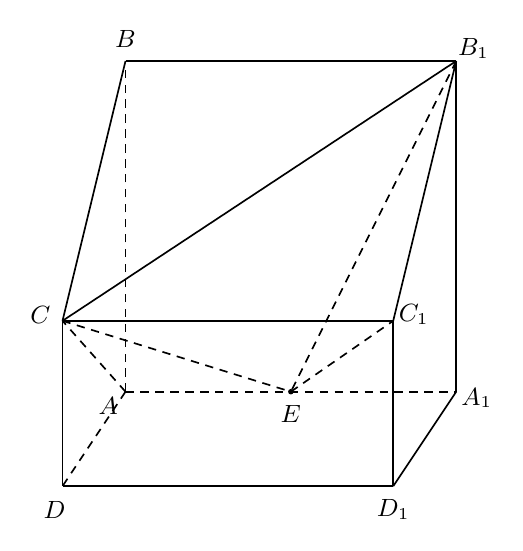
\begin{tikzpicture}[
  x=1cm, y=1cm,
  every node/.style={font=\small, inner sep=1pt},
  s/.style={line width=0.6pt},
  d/.style={line width=0.6pt, dash pattern=on 3.0pt off 2.4pt},
]

  % ---------- 实线 ----------
  \draw[s] (0,0) -- (0,2.10);          % D-C
  \draw[s] (0,2.10) -- (4.20,2.10);    % C-C1
  \draw[s] (4.20,2.10) -- (4.20,0);    % C1-D1
  \draw[s] (4.20,0) -- (0,0);          % D1-D

  \draw[s] (0,2.10) -- (0.80,5.40);    % C-B
  \draw[s] (0.80,5.40) -- (5.00,5.40); % B-B1
  \draw[s] (5.00,5.40) -- (4.20,2.10); % B1-C1
  \draw[s] (5.00,5.40) -- (5.00,1.20); % B1-A1
  \draw[s] (5.00,1.20) -- (4.20,0);    % A1-D1
  \draw[s] (5.00,5.40) -- (0,2.10);    % B1-C

  % ---------- 虚线 ----------
  \draw[d] (0.80,1.20) -- (0.80,5.40); % A-B
  \draw[d] (0.80,1.20) -- (0,0);       % A-D
  \draw[d] (0.80,1.20) -- (5.00,1.20); % A-A1（过 E）
  \draw[d] (0.80,1.20) -- (0,2.10);    % A-C
  \draw[d] (0,2.10) -- (2.90,1.20);    % C-E
  \draw[d] (2.90,1.20) -- (4.20,2.10); % E-C1
  \draw[d] (5.00,5.40) -- (2.90,1.20); % B1-E（原页辅助线）

  % E 点
  \fill (2.90,1.20) circle [radius=0.035];

  % ---------- 标签 ----------
  \node at (0.58,1.02) {$A$};
  \node at (0.80,5.68) {$B$};
  \node at (-0.28,2.18) {$C$};
  \node at (4.46,2.18) {$C_1$};
  \node at (-0.10,-0.30) {$D$};
  \node at (4.20,-0.30) {$D_1$};
  \node at (5.26,1.12) {$A_1$};
  \node at (5.22,5.56) {$B_1$};
  \node at (2.90,0.92) {$E$};

\end{tikzpicture}
\end{center}
\nopagebreak[4]
\Needspace{4\baselineskip}
\textbf{解析}
\Needspace{5\baselineskip}
\textbf{（1）} 以 $A$ 为原点，$AB$，$AD$，$AA_1$ 所在直线分别为 $x$，$y$，$z$ 轴建立空间直角坐标系。由 $AB\parallel DC$，$AB\perp AD$，$AD=CD=1$，$AB=AA_1=2$，得
\nopagebreak[4]
\[A(0,0,0),\quad B(2,0,0),\quad D(0,1,0),\quad C(1,1,0),\]
\nopagebreak[4]
\[A_1(0,0,2),\quad B_1(2,0,2),\quad C_1(1,1,2),\quad D_1(0,1,2).\]
\Needspace{5\baselineskip}
$E$ 为 $AA_1$ 的中点，故
\nopagebreak[4]
\[E(0,0,1).\]
\Needspace{5\baselineskip}
于是
\nopagebreak[4]
\[\overrightarrow{B_1C_1}=(-1,1,0),\qquad
\overrightarrow{CE}=E-C=(-1,-1,1).\]
\Needspace{5\baselineskip}
计算内积：
\nopagebreak[4]
\[\overrightarrow{B_1C_1}\cdot\overrightarrow{CE}
=(-1)(-1)+1\cdot(-1)+0\cdot1=1-1=0.\]
\Needspace{5\baselineskip}
故
\nopagebreak[4]
\[B_1C_1\perp CE.\]

\Needspace{5\baselineskip}
\textbf{（2）} 平面 $B_1CE$ 内两向量
\nopagebreak[4]
\[\overrightarrow{CB_1}=(1,-1,2),\qquad
\overrightarrow{CE}=(-1,-1,1).\]
\Needspace{5\baselineskip}
取法向量
\nopagebreak[4]
\[\boldsymbol n_1=\overrightarrow{CB_1}\times\overrightarrow{CE}
=\begin{vmatrix}
\boldsymbol i&\boldsymbol j&\boldsymbol k\\
1&-1&2\\
-1&-1&1
\end{vmatrix}
=(1,-3,-2).\]
\Needspace{5\baselineskip}
平面 $C_1CE$ 内两向量
\nopagebreak[4]
\[\overrightarrow{CC_1}=(0,0,2),\qquad
\overrightarrow{CE}=(-1,-1,1).\]
\Needspace{5\baselineskip}
取法向量
\nopagebreak[4]
\[\boldsymbol n_2=\overrightarrow{CC_1}\times\overrightarrow{CE}
=\begin{vmatrix}
\boldsymbol i&\boldsymbol j&\boldsymbol k\\
0&0&2\\
-1&-1&1
\end{vmatrix}
=(2,-2,0).\]
\Needspace{5\baselineskip}
设二面角的平面角为 $\theta$，则
\nopagebreak[4]
\[\cos\theta
=\frac{|\boldsymbol n_1\cdot\boldsymbol n_2|}{|\boldsymbol n_1||\boldsymbol n_2|}
=\frac{|2+6+0|}{\sqrt{1+9+4}\cdot\sqrt{4+4}}
=\frac{8}{2\sqrt{28}}
=\frac{2}{\sqrt7}.\]
\Needspace{5\baselineskip}
故
\nopagebreak[4]
\[\sin\theta=\sqrt{1-\cos^2\theta}
=\sqrt{1-\frac47}
=\sqrt{\frac37}
=\frac{\sqrt{21}}7.\]

\Needspace{5\baselineskip}
\textbf{（3）} 点 $M$ 在线段 $C_1E$ 上，设
\nopagebreak[4]
\[\overrightarrow{EM}=t\overrightarrow{EC_1}\quad(0\leqslant t\leqslant1).\]
\Needspace{5\baselineskip}
由 $E(0,0,1)$，$C_1(1,1,2)$ 得
\nopagebreak[4]
\[M(t,t,1+t).\]
\Needspace{5\baselineskip}
平面 $ADD_1A_1$ 即 $x=0$，其法向量可取 $\boldsymbol n=(1,0,0)$。直线 $AM$ 的方向向量为
\nopagebreak[4]
\[\overrightarrow{AM}=(t,t,1+t).\]
\Needspace{5\baselineskip}
设直线 $AM$ 与平面 $ADD_1A_1$ 所成角为 $\varphi$，则
\nopagebreak[4]
\[\sin\varphi
=\frac{|\overrightarrow{AM}\cdot\boldsymbol n|}{|\overrightarrow{AM}||\boldsymbol n|}
=\frac{t}{\sqrt{t^2+t^2+(1+t)^2}}
=\frac{t}{\sqrt{3t^2+2t+1}}.\]
\Needspace{5\baselineskip}
由题设 $\sin\varphi=\dfrac{\sqrt2}{6}$，得
\nopagebreak[4]
\[\frac{t^2}{3t^2+2t+1}=\frac1{18}.\]
\Needspace{5\baselineskip}
去分母：
\nopagebreak[4]
\[18t^2=3t^2+2t+1\Longrightarrow 15t^2-2t-1=0.\]
\Needspace{5\baselineskip}
解得
\nopagebreak[4]
\[t=\frac{2\pm\sqrt{4+60}}{30}=\frac{2\pm8}{30},\]
即 $t=\dfrac13$ 或 $t=-\dfrac15$。因 $0\leqslant t\leqslant1$，取 $t=\dfrac13$。

\Needspace{5\baselineskip}
于是
\nopagebreak[4]
\[|\overrightarrow{AM}|=\sqrt{3\cdot\frac19+2\cdot\frac13+1}
=\sqrt{\frac13+\frac23+1}=\sqrt2.\]
故线段 $AM$ 的长为 $\sqrt2$。

\gkanswer{答案（1）：证明见解析。取 $A$ 为原点建系，$\overrightarrow{B_1C_1}=(-1,1,0)$，$\overrightarrow{CE}=(-1,-1,1)$，内积为 $0$。}

\gkanswer{答案（2）：$\dfrac{\sqrt{21}}7$。两平面法向量可取 $\boldsymbol n_1=(1,-3,-2)$，$\boldsymbol n_2=(2,-2,0)$，故 $\cos\theta=\dfrac2{\sqrt7}$，$\sin\theta=\dfrac{\sqrt{21}}7$。}

\gkanswer{答案（3）：$\sqrt2$。设 $M(t,t,1+t)$，由 $\dfrac{t}{\sqrt{3t^2+2t+1}}=\dfrac{\sqrt2}{6}$ 得 $15t^2-2t-1=0$，取 $t=\dfrac13$，故 $AM=\sqrt2$。}

\end{answer}
\begin{answer}
\gksolhead{18}{}

\textbf{题目}：

设椭圆 $\dfrac{x^2}{a^2}+\dfrac{y^2}{b^2}=1$（$a>b>0$）的左焦点为 $F$，离心率为 $\dfrac{\sqrt3}{3}$，过点 $F$ 且与 $x$ 轴垂直的直线被椭圆截得的线段长为 $\dfrac{4\sqrt3}{3}$。

（1） 求椭圆的方程；

（2） 设 $A$，$B$ 分别为椭圆的左、右顶点，过点 $F$ 且斜率为 $k$ 的直线与椭圆交于 $C$，$D$ 两点。若 $\overrightarrow{AC}\cdot\overrightarrow{DB}+\overrightarrow{AD}\cdot\overrightarrow{CB}=8$，求 $k$ 的值。

\Needspace{4\baselineskip}
\textbf{解析}
\Needspace{5\baselineskip}
\textbf{（1）} 设焦距为 $2c$。由离心率
\nopagebreak[4]
\[e=\frac ca=\frac{\sqrt3}{3},\]
\Needspace{5\baselineskip}
得
\nopagebreak[4]
\[c^2=\frac{a^2}{3},\qquad b^2=a^2-c^2=\frac{2a^2}{3}.\]
\Needspace{5\baselineskip}
左焦点为 $F(-c,0)$。过 $F$ 且垂直于 $x$ 轴的直线为 $x=-c$，代入椭圆方程：
\nopagebreak[4]
\[\frac{c^2}{a^2}+\frac{y^2}{b^2}=1
\Longrightarrow \frac{y^2}{b^2}=1-\frac13=\frac23
\Longrightarrow y^2=\frac{2b^2}{3}.\]
\Needspace{5\baselineskip}
截得线段长为
\nopagebreak[4]
\[2|y|=2b\sqrt{\frac23}=\frac{4\sqrt3}{3}.\]
\Needspace{5\baselineskip}
两边平方：
\nopagebreak[4]
\[4b^2\cdot\frac23=\frac{16}{3}\Longrightarrow b^2=2.\]
\Needspace{5\baselineskip}
从而
\nopagebreak[4]
\[a^2=\frac32b^2=3,\qquad c^2=1.\]
\Needspace{5\baselineskip}
椭圆方程为
\nopagebreak[4]
\[\frac{x^2}{3}+\frac{y^2}{2}=1.\]

\Needspace{5\baselineskip}
\textbf{（2）} 由（1），$A(-\sqrt3,0)$，$B(\sqrt3,0)$，$F(-1,0)$。过 $F$ 且斜率为 $k$ 的直线为
\nopagebreak[4]
\[y=k(x+1).\]
\Needspace{5\baselineskip}
代入椭圆方程：
\nopagebreak[4]
\[\frac{x^2}{3}+\frac{k^2(x+1)^2}{2}=1.\]
\Needspace{5\baselineskip}
两边乘以 $6$：
\nopagebreak[4]
\[2x^2+3k^2(x+1)^2=6,\]
\Needspace{5\baselineskip}
即
\nopagebreak[4]
\[(2+3k^2)x^2+6k^2x+3k^2-6=0.\]
\Needspace{5\baselineskip}
设交点 $C(x_1,y_1)$，$D(x_2,y_2)$，则由韦达定理
\nopagebreak[4]
\[x_1+x_2=-\frac{6k^2}{2+3k^2},\qquad
x_1x_2=\frac{3k^2-6}{2+3k^2}.\]
\Needspace{5\baselineskip}
又 $y_i=k(x_i+1)$，故
\nopagebreak[4]
\[y_1y_2=k^2(x_1+1)(x_2+1)
=k^2\bigl[x_1x_2+(x_1+x_2)+1\bigr].\]

\Needspace{5\baselineskip}
计算题设中的数量积。由
\nopagebreak[4]
\[\overrightarrow{AC}=(x_1+\sqrt3,y_1),\qquad
\overrightarrow{DB}=(\sqrt3-x_2,-y_2),\]
\nopagebreak[4]
\[\overrightarrow{AD}=(x_2+\sqrt3,y_2),\qquad
\overrightarrow{CB}=(\sqrt3-x_1,-y_1),\]
\Needspace{5\baselineskip}
得
\nopagebreak[4]
\[\begin{aligned}
&\overrightarrow{AC}\cdot\overrightarrow{DB}
+\overrightarrow{AD}\cdot\overrightarrow{CB}\\
&=(x_1+\sqrt3)(\sqrt3-x_2)-y_1y_2
+(x_2+\sqrt3)(\sqrt3-x_1)-y_1y_2\\
&=\bigl[6-2x_1x_2\bigr]-2y_1y_2\\
&=6-2(x_1x_2+y_1y_2).
\end{aligned}\]
\Needspace{5\baselineskip}
由题设该值为 $8$，得
\nopagebreak[4]
\[6-2(x_1x_2+y_1y_2)=8
\Longrightarrow x_1x_2+y_1y_2=-1.\]
\Needspace{5\baselineskip}
而
\nopagebreak[4]
\[\begin{aligned}
x_1x_2+y_1y_2
&=(1+k^2)x_1x_2+k^2(x_1+x_2)+k^2\\
&=\frac{(1+k^2)(3k^2-6)-6k^4+k^2(2+3k^2)}{2+3k^2}\\
&=\frac{-k^2-6}{2+3k^2}.
\end{aligned}\]
\Needspace{5\baselineskip}
于是
\nopagebreak[4]
\[\frac{-k^2-6}{2+3k^2}=-1
\Longrightarrow -k^2-6=-2-3k^2
\Longrightarrow 2k^2=4
\Longrightarrow k^2=2.\]
\Needspace{5\baselineskip}
故
\nopagebreak[4]
\[k=\pm\sqrt2.\]

\gkanswer{答案（1）：$\dfrac{x^2}{3}+\dfrac{y^2}{2}=1$。由 $e=\dfrac{\sqrt3}{3}$ 得 $b^2=\dfrac23a^2$；通径长 $\dfrac{4\sqrt3}{3}$ 给出 $b^2=2$，$a^2=3$。}

\gkanswer{答案（2）：$k=\pm\sqrt2$。联立直线 $y=k(x+1)$ 与椭圆，韦达定理代入 $\overrightarrow{AC}\cdot\overrightarrow{DB}+\overrightarrow{AD}\cdot\overrightarrow{CB}=6-2(x_1x_2+y_1y_2)=8$，得 $k^2=2$。}

\end{answer}
\begin{answer}
\gksolhead{19}{}

\textbf{题目}：

已知首项为 $\dfrac32$ 的等比数列 $\{a_n\}$ 不是递减数列，其前 $n$ 项和为 $S_n$（$n\in\mathbf{N}^{*}$），且 $S_3+a_3$，$S_5+a_5$，$S_4+a_4$ 成等差数列。

（1） 求数列 $\{a_n\}$ 的通项公式；

（2） 设 $T_n=S_n-\dfrac{1}{S_n}$（$n\in\mathbf{N}^{*}$），求数列 $\{T_n\}$ 的最大项的值与最小项的值。

\Needspace{4\baselineskip}
\textbf{解析}
\textbf{（1）} 设等比数列的公比为 $q$，首项 $a_1=\dfrac32$。

\Needspace{5\baselineskip}
若 $q=1$，则 $a_n=\dfrac32$，$S_n=\dfrac{3n}{2}$，于是
\nopagebreak[4]
\[S_3+a_3=6,\qquad S_5+a_5=9,\qquad S_4+a_4=\frac{15}{2},\]
不满足 $2(S_5+a_5)=(S_3+a_3)+(S_4+a_4)$，故 $q\neq1$。

\Needspace{5\baselineskip}
当 $q\neq1$ 时，
\nopagebreak[4]
\[S_n=\frac32\cdot\frac{1-q^n}{1-q},\qquad a_n=\frac32q^{n-1},\]
\Needspace{5\baselineskip}
所以
\nopagebreak[4]
\[S_n+a_n=\frac32\left(\frac{1-q^n}{1-q}+q^{n-1}\right).\]
\Needspace{5\baselineskip}
由 $S_3+a_3$，$S_5+a_5$，$S_4+a_4$ 成等差数列，
\nopagebreak[4]
\[2(S_5+a_5)=(S_3+a_3)+(S_4+a_4).\]
\Needspace{5\baselineskip}
两边乘以 $\dfrac{2(1-q)}{3}$，整理得
\nopagebreak[4]
\[2(1-q^5+q^4-q^5)
-(1-q^3+q^2-q^3)
-(1-q^4+q^3-q^4)=0.\]
\Needspace{5\baselineskip}
合并同类项：
\nopagebreak[4]
\[-4q^5+4q^4+q^3-q^2=0,\]
\Needspace{5\baselineskip}
即
\nopagebreak[4]
\[q^2(4q^2-1)=0\quad(q\neq1).\]
\Needspace{5\baselineskip}
因 $q\neq0$，故
\nopagebreak[4]
\[q=\pm\frac12.\]

若 $q=\dfrac12$，则 $a_n=\dfrac32\left(\dfrac12\right)^{n-1}>0$ 且随 $n$ 增大而减小，是递减数列，与题设“不是递减数列”矛盾，舍去。

\Needspace{5\baselineskip}
故 $q=-\dfrac12$，通项为
\nopagebreak[4]
\[a_n=\frac32\left(-\frac12\right)^{n-1}
=\frac{3(-1)^{n-1}}{2^n}\quad(n\in\mathbf N^*).\]

\Needspace{5\baselineskip}
\textbf{（2）} 由（1），
\nopagebreak[4]
\[S_n=\frac{\frac32\left[1-\left(-\frac12\right)^n\right]}{1+\frac12}
=1-\left(-\frac12\right)^n.\]
\Needspace{5\baselineskip}
记 $u_n=\left(-\dfrac12\right)^n$，则 $S_n=1-u_n$，且
\nopagebreak[4]
\[T_n=S_n-\frac1{S_n}.\]
\Needspace{5\baselineskip}
函数
\nopagebreak[4]
\[\varphi(S)=S-\frac1S\]
\Needspace{5\baselineskip}
在 $S>0$ 上单调递增，因为
\nopagebreak[4]
\[\varphi'(S)=1+\frac1{S^2}>0.\]

\Needspace{5\baselineskip}
当 $n$ 为偶数时，$u_n=2^{-n}>0$，
\nopagebreak[4]
\[S_n=1-2^{-n},\]
\Needspace{5\baselineskip}
随 $n$ 增大而增大，故 $T_n$ 随偶数 $n$ 增大而增大。偶数项中最小者为
\nopagebreak[4]
\[T_2=S_2-\frac1{S_2}=\frac34-\frac43=-\frac7{12},\]
且 $T_n<0$ 而 $T_n\to0$（$n$ 为偶数，$n\to\infty$）。

\Needspace{5\baselineskip}
当 $n$ 为奇数时，$u_n=-2^{-n}<0$，
\nopagebreak[4]
\[S_n=1+2^{-n},\]
\Needspace{5\baselineskip}
随 $n$ 增大而减小，故 $T_n$ 随奇数 $n$ 增大而减小。奇数项中最大者为
\nopagebreak[4]
\[T_1=S_1-\frac1{S_1}=\frac32-\frac23=\frac56,\]
且 $T_n>0$ 而 $T_n\to0$（$n$ 为奇数，$n\to\infty$）。

\Needspace{5\baselineskip}
因此 $\{T_n\}$ 的最大项为
\nopagebreak[4]
\[T_1=\frac56,\]
\Needspace{5\baselineskip}
最小项为
\nopagebreak[4]
\[T_2=-\frac7{12}.\]

\gkanswer{答案（1）：$a_n=\dfrac{3(-1)^{n-1}}{2^n}$（$n\in\mathbf N^*$）。由等差条件得 $q^2(4q^2-1)=0$，即 $q=\pm\dfrac12$；$q=\dfrac12$ 时为递减数列，舍去，故 $q=-\dfrac12$。}

\gkanswer{答案（2）：最大项 $T_1=\dfrac56$，最小项 $T_2=-\dfrac7{12}$。$S_n=1-\left(-\dfrac12\right)^n$；偶数项 $T_n$ 递增，奇数项 $T_n$ 递减，且分别以 $0$ 为极限。}

\end{answer}
\begin{answer}
\gksolhead{20}{}

\textbf{题目}：

已知函数 $f(x)=x^2\ln x$。

（1） 求函数 $f(x)$ 的单调区间；

（2） 证明：对任意的 $t>0$，存在唯一的 $s$，使 $t=f(s)$；

\Needspace{5\baselineskip}
（3） 设（2）中所确定的 $s$ 关于 $t$ 的函数为 $s=g(t)$，证明：当 $t>e^2$ 时，有
\nopagebreak[4]
\[\frac25<\frac{\ln g(t)}{\ln t}<\frac12.\]

\Needspace{4\baselineskip}
\textbf{解析}
\Needspace{5\baselineskip}
\textbf{（1）} 定义域为 $x>0$。求导：
\nopagebreak[4]
\[f'(x)=2x\ln x+x^2\cdot\frac1x=x(2\ln x+1).\]
\Needspace{5\baselineskip}
由 $x>0$，$f'(x)$ 的符号由 $2\ln x+1$ 决定：
\nopagebreak[4]
\[f'(x)<0\Longleftrightarrow 0<x<e^{-\frac12},\qquad
f'(x)>0\Longleftrightarrow x>e^{-\frac12}.\]
\Needspace{5\baselineskip}
故 $f(x)$ 的单调递减区间为
\nopagebreak[4]
\[\left(0,e^{-\frac12}\right),\]
\Needspace{5\baselineskip}
单调递增区间为
\nopagebreak[4]
\[\left(e^{-\frac12},+\infty\right).\]

\Needspace{5\baselineskip}
\textbf{（2）} 由（1），$f$ 在 $\left(e^{-\frac12},+\infty\right)$ 上连续且严格递增，并且
\nopagebreak[4]
\[f\left(e^{-\frac12}\right)
=e^{-1}\ln e^{-\frac12}
=-\frac1{2e}<0,\qquad
\lim_{x\to+\infty}f(x)=+\infty.\]
\Needspace{5\baselineskip}
因此 $f$ 在该区间上的值域为
\nopagebreak[4]
\[\left[-\frac1{2e},+\infty\right).\]
对任意 $t>0$，因 $0>-\dfrac1{2e}$，故 $t$ 属于上述值域，存在 $s\in\left(e^{-\frac12},+\infty\right)$ 使 $f(s)=t$；又 $f$ 在该区间上严格递增，这样的 $s$ 唯一。

另一方面，在 $\left(0,e^{-\frac12}\right)$ 上 $f(x)<0$，不可能等于 $t>0$。所以对任意 $t>0$，存在唯一的 $s$，使 $t=f(s)$。

\Needspace{5\baselineskip}
\textbf{（3）} 由（2），$s=g(t)$ 是方程
\nopagebreak[4]
\[t=s^2\ln s\]
在 $\left(e^{-\frac12},+\infty\right)$ 上的唯一解，且 $f$ 在该区间上严格递增。

\Needspace{5\baselineskip}
先证 $s>e$。因为
\nopagebreak[4]
\[f(e)=e^2\ln e=e^2,\]
\Needspace{5\baselineskip}
且 $t>e^2=f(e)$，由 $f$ 在 $\left(e^{-\frac12},+\infty\right)$ 上严格递增，得
\nopagebreak[4]
\[s>e.\]
从而 $s$，$\sqrt t$，$t^{\frac25}$ 都落在 $f$ 的严格递增区间 $\left(e^{-\frac12},+\infty\right)$ 内。

\Needspace{5\baselineskip}
\textbf{上界。} 因为 $t>e^2$，所以 $\ln t>2$。于是
\nopagebreak[4]
\[f(\sqrt t)=t\ln\sqrt t=\frac t2\ln t>t=f(s).\]
\Needspace{5\baselineskip}
由 $f$ 严格递增，得
\nopagebreak[4]
\[\sqrt t>s,\]
\Needspace{5\baselineskip}
两边取对数：
\nopagebreak[4]
\[\frac12\ln t>\ln s
\Longrightarrow \frac{\ln s}{\ln t}<\frac12.\]

\Needspace{5\baselineskip}
\textbf{下界。} 令 $u=t^{\frac15}$。由 $t>e^2$ 得
\nopagebreak[4]
\[u>e^{\frac25}.\]
\Needspace{5\baselineskip}
考察函数
\nopagebreak[4]
\[\psi(u)=u-2\ln u\quad(u>0).\]
\Needspace{5\baselineskip}
求导：
\nopagebreak[4]
\[\psi'(u)=1-\frac2u,\]
\Needspace{5\baselineskip}
故 $\psi$ 在 $(0,2)$ 上递减，在 $(2,+\infty)$ 上递增，最小值为
\nopagebreak[4]
\[\psi(2)=2-2\ln2>0.\]
\Needspace{5\baselineskip}
所以对一切 $u>0$ 都有
\nopagebreak[4]
\[u>2\ln u.\]
\Needspace{5\baselineskip}
取 $u=t^{\frac15}$，得
\nopagebreak[4]
\[\frac25\ln t=2\ln u<u=t^{\frac15}.\]
\Needspace{5\baselineskip}
两边乘以 $t^{\frac45}>0$：
\nopagebreak[4]
\[\frac25t^{\frac45}\ln t<t.\]
\Needspace{5\baselineskip}
而
\nopagebreak[4]
\[f\left(t^{\frac25}\right)
=\left(t^{\frac25}\right)^2\ln\left(t^{\frac25}\right)
=t^{\frac45}\cdot\frac25\ln t
<\ t=f(s).\]
\Needspace{5\baselineskip}
由 $f$ 严格递增，得
\nopagebreak[4]
\[t^{\frac25}<s.\]
\Needspace{5\baselineskip}
两边取对数：
\nopagebreak[4]
\[\frac25\ln t<\ln s
\Longrightarrow \frac{\ln s}{\ln t}>\frac25.\]

\Needspace{5\baselineskip}
综上，当 $t>e^2$ 时，
\nopagebreak[4]
\[\frac25<\frac{\ln g(t)}{\ln t}<\frac12.\]

数值复核：用二分法解 $s^2\ln s=t$，取 $t=e^4,e^5,e^{10}$，得

\begin{center}
\begin{tabular}{lll}
\toprule
$t$ & $s=g(t)$ & $\dfrac{\ln g(t)}{\ln t}$ \\
\midrule
$e^4\approx54.598150$ & $5.622916116$ & $0.431712603$ \\
$e^5\approx148.413159$ & $8.360125363$ & $0.424694685$ \\
$e^{10}\approx22026.465795$ & $71.790613216$ & $0.427375373$ \\
\bottomrule
\end{tabular}
\end{center}

三者的比值都在 $\left(\dfrac25,\dfrac12\right)$ 内，与证明一致。

\gkanswer{答案（1）：单调递减区间 $\left(0,e^{-\frac12}\right)$，单调递增区间 $\left(e^{-\frac12},+\infty\right)$。由 $f'(x)=x(2\ln x+1)$ 判号即得。}

\gkanswer{答案（2）：证明见解析。$f$ 在 $\left(e^{-\frac12},+\infty\right)$ 上严格递增，值域为 $\left[-\dfrac1{2e},+\infty\right)$，而 $t>0>-\dfrac1{2e}$，故存在唯一解；另一段 $f<0$ 不产生解。}

\gkanswer{答案（3）：证明见解析。由 $t>e^2=f(e)$ 得 $s>e$；比较 $f(\sqrt t)=\dfrac t2\ln t>t$ 得 $\sqrt t>s$，给出上界；比较 $f\left(t^{\frac25}\right)=\dfrac25t^{\frac45}\ln t<t$ 得 $t^{\frac25}<s$，给出下界。数值复核 $t=e^4,e^5,e^{10}$ 时比值分别约为 $0.4317$，$0.4247$，$0.4274$，均落在 $\left(\dfrac25,\dfrac12\right)$ 内。}

\end{answer}